
\section{Метрики}
\label{sec:metrics}

Данный раздел посвящен выявлению особенностей и численному сравнению алгоритмов. В последующих разделах везде подразумеваются следующие обозначения:

\begin{itemize}
    \item $R_k$ - поиск, реализующий алгоритм \textit{BM25} \cite{robertson2009probabilistic}
    \item $R_e$ - поиск ближайшего соседа (ANN), использующий реализацию \textit{Weavaite} \cite{weaviate} алгоритмом \textit{HNSW} \url{enwiki:hsnw}
    \item $R_h$ - гибридный поиск, совмещающий первых два подхода, с наилучшим выбранным порогом $\theta$.
    \item $R_{\gamma}$ - поиск ближайшего соседа (ANN), используюший ранжирование $f(\gamma_1, \gamma_2)$ \eqref{eq:gamma-func}
\end{itemize}


\subsection{Выбор ключевых слов}
\label{sec:keywords-vs-content}

Для функции ранжирования, вполне мог бы подойти и сам текст параграфа. Действительно, код и оставшаяся часть алгоритма никак бы не изменились. 
Однако выбор самого текста параграфа влечет за собой некоторые изъяны, и как показано на графике ниже, аномальные всплески сильно ``ухудшают'' общую метрику, 
приоритезируя выдачу по ключевым словам. Так, например, для набора данных $D_u$ показано сравнения $\phi_r$ на контексте документа и его ключевых словах:

% \begin{figure}[ht]
%     \centering
%     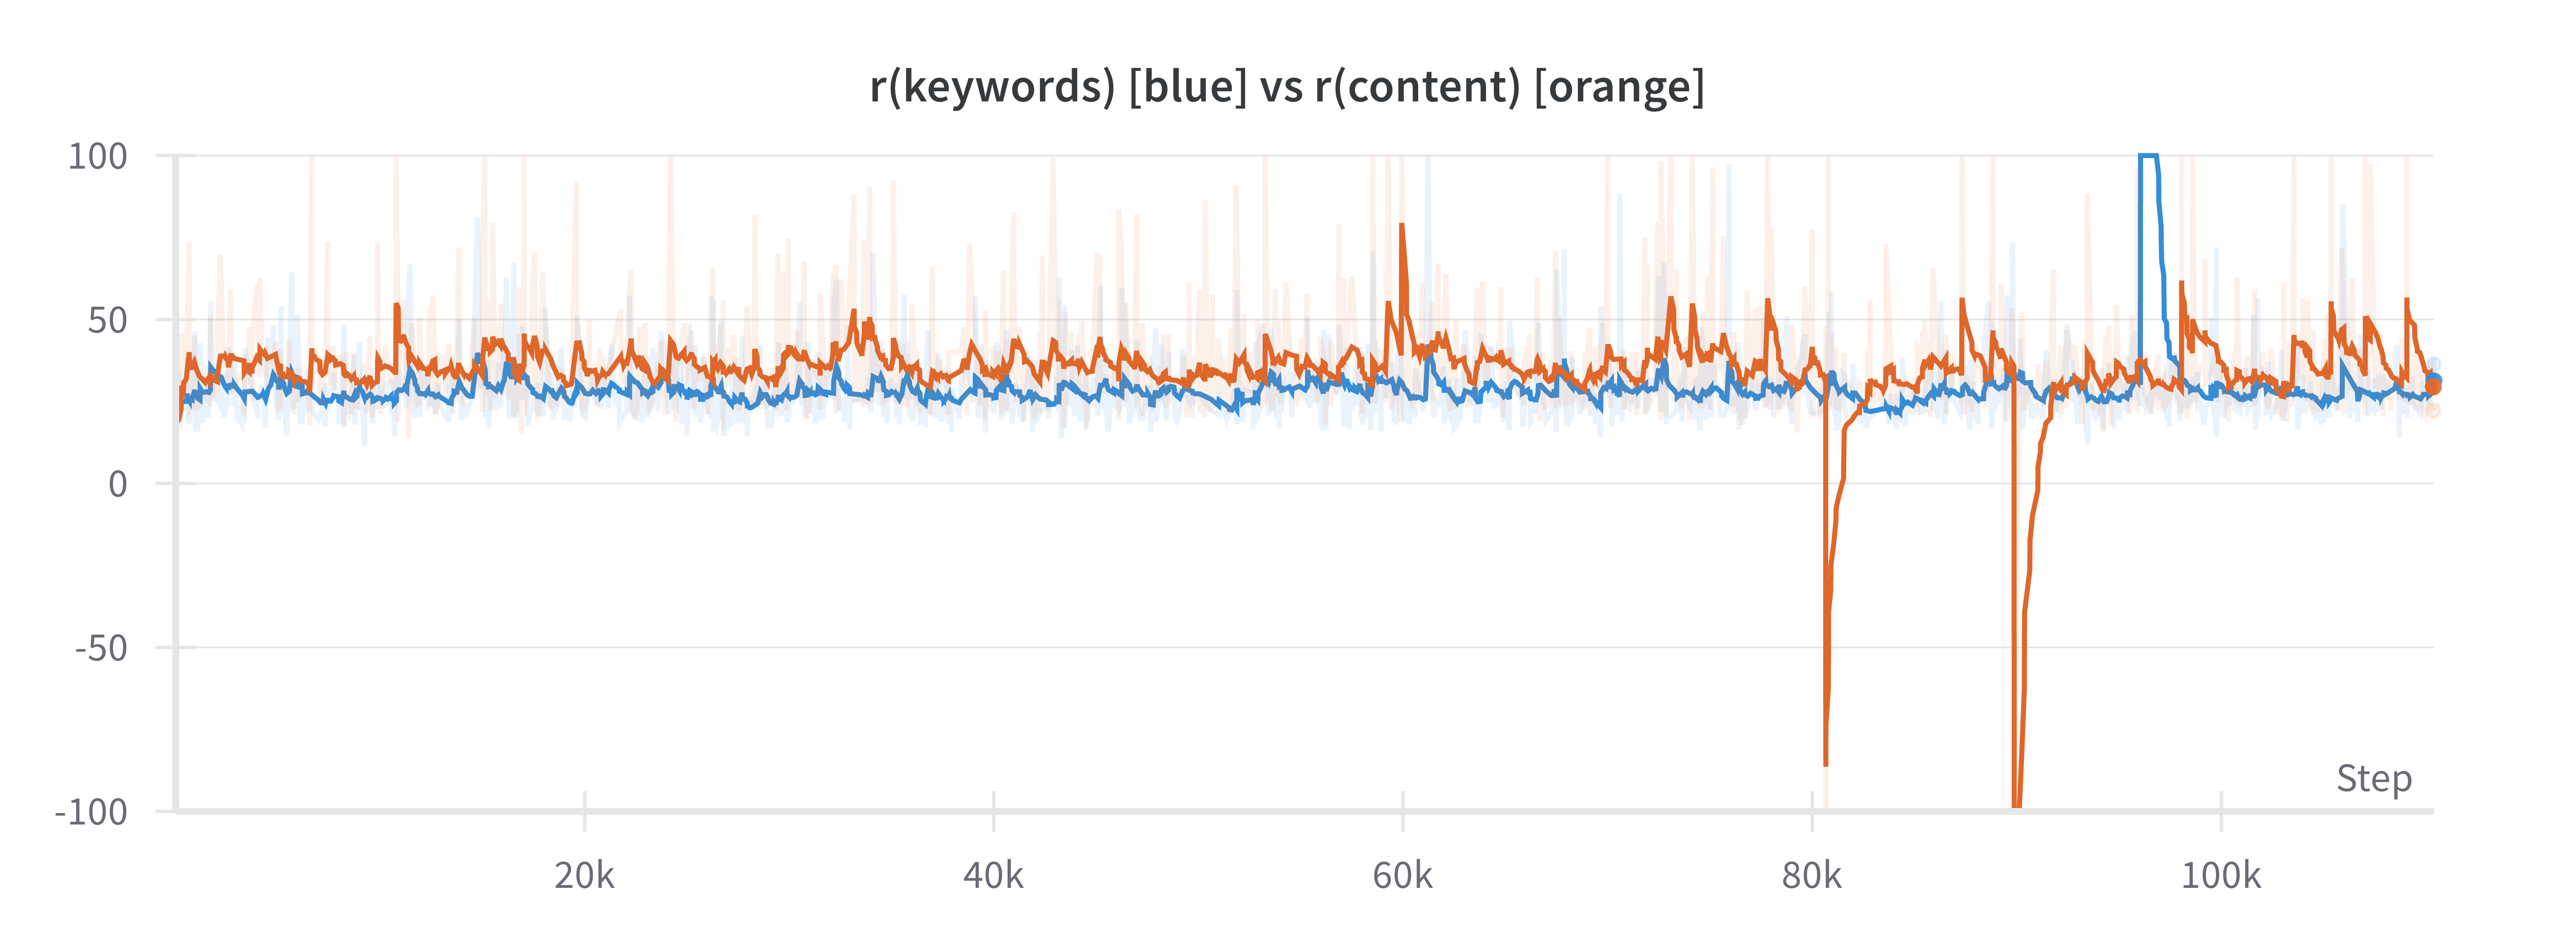
\includegraphics[width=\columnwidth]{figures/idf-recall-content-vs-keywords.png} % Используем ширину одной колонки
%     \caption{Comparison of $\phi_r$ using $D_u$ dataset}
%     \label{fig:comparison-phir-content-vs-keywords}
% \end{figure}


\subsection{Результаты}
\label{sec:final-metrics}

Ниже, приведены основные результаты сравнения, подтверждающие гипотезу о том, что гибридный поиск $R_h$(с наилучшим коэффициентом $\theta$) 
показывает результаты хуже, чем предложенный в статье алгоритм - $R_{\gamma}$, основанный на дополнительном ранжировании, выбирающий $top_p$ и дополнительно 
ранжирующий результаты через $\gamma_1, \gamma_2$.

В таблицах ~\ref{tab:hitrate-small} ~\ref{tab:hitrate-base} ~\ref{tab:hitrate-large} представлены результаты сравнения на выборке данных из $D_u$, $D_v$ для моделей семейства \textit{E5} \cite{e5} размеров \textit{$E5_{small}$}, \textit{$E5_{ base}$} и \textit{$E5_{large}$} соответственно.
\begin{table}[ht]
    \centering
    \begin{tabular}{lcccccc}
        \hline
        & \textbf{HitRate@k (\(D_u\))} & \textbf{HitRate@k (\(D_v\))} \\
       \hline
       \(R_k\)      &  0.49&  0.79 \\
       \(R_e\)      &  0.53&  0.89\\
       \(R_h\)      &  0.56&  0.91\\
       \(R_{\gamma}\) &  \textbf{0.60}&  \textbf{0.93}\\
       \hline
       \end{tabular}
    \caption{Метрика $HitRate@k$ на примере модели $E5_{small}$ \cite{e5}}
    \label{tab:hitrate-small}
\end{table}
\begin{table}[ht]
    \centering
    \begin{tabular}{lcccccc}
        \hline
        & \textbf{HitRate@k (\(D_u\))} & \textbf{HitRate@k (\(D_v\))} \\
       \hline
       \(R_k\)      &  0.49&  0.79 \\
       \(R_e\)      &  0.58&  0.90\\
       \(R_h\)      &  0.61&  0.92\\
       \(R_{\gamma}\) &  \textbf{0.633}&  \textbf{0.93}\\
       \hline
       \end{tabular}
    \caption{Метрика $HitRate@k$ на примере модели $E5_{base}$ \cite{e5}}
    \label{tab:hitrate-base}
\end{table}
\begin{table}[ht]
    \centering
    \begin{tabular}{lcccccc}
        \hline
        & \textbf{HitRate@k (\(D_u\))} & \textbf{HitRate@k (\(D_v\))} \\
       \hline
       \(R_k\)      &  0.49&  0.79 \\
       \(R_e\)      &  0.64&  0.92\\
       \(R_h\)      &  0.66&  0.93\\
       \(R_{\gamma}\) &  \textbf{0.681}&  \textbf{0.94}\\
       \hline
       \end{tabular}
    \caption{Метрика $HitRate@k$ на примере модели $E5_{large}$ \cite{e5}}
    \label{tab:hitrate-large}
\end{table}

\noindent
\textbf{Universe Question ($D_u$)}~\cite{repojustatom} - вопросы и параграфы, основанные на вселенных из книг, игр, фильмов или сериалов.
Набор данных был составлен экспертами, которые были погружены в эти вселенные. Помимо уникальной лингвистической структуры, речевыми оборотами, 
этот датасет предсталяет особую трудность для адаптации из-за сложности в токенизации имен собственных, заклинаний и лексическим сдвигом от формального повествования. 
Так, например, в таких произведениях как 
\href{https://en.wikipedia.org/wiki/Harry_Potter}{Harry Potter}, 
\href{https://en.wikipedia.org/wiki/The_Witcher}{The Witcher}, 
\href{https://en.wikipedia.org/wiki/The_Hunger_Games}{The Hunger Games} и других 
существует существенный сдвиг в сторону фэнтезийных терминов, которые токенизируются буквально по слогам, что приводит к ``сдвинутому распределению''. В таблице 
~\ref{tab:queries_DU} приведены примеры вопросов.
\begin{table}[ht]
    \centering
    \small
    \caption{$D_u$ sampled queries}
    \label{tab:queries_DU}
    \begin{tabular}{p{0.45\linewidth} p{0.45\linewidth}}
    \toprule
    \textbf{Query} & \textbf{Universe} \\
    \midrule
    In the novel 'Crime and Punishment', how does Raskolnikov feel about the squalid conditions of his living space? & Crime and Punishment \\
    \midrule
    Why do Katniss and Gale choose to trade with Greasy Sae despite potentially better deals available in the 'Hunger Games' universe?      & Hunger Games\\
    \midrule
    Почему Катон злится на трибута из Дистрикта-3 и безжалостно убивает его после взрыва мин? & Hunger Games \\
    \midrule
    Какую речь произносит мэр во время Жатвы, когда часы на ратуше пробивают два?      & Hunger Games \\
    \midrule
    In the book 'Harry Potter and the Prisoner of Azkaban', what transformation occurs to Ron Weasley's rat when Black and Lupin simultaneously aim their wands and cast a spell?          & Harry Potter and the Prisoner of Azkaban \\
    \midrule
    What motivates Harry Potter to continue practicing the Patronus charm despite the challenges presented in the universe of 'Harry Potter and the Prisoner of Azkaban'?          & Harry Potter and the Prisoner of Azkaban \\
    \bottomrule
    \end{tabular}
\end{table}



\noindent
\textbf{Vanilla factoid Question ($D_v$)}~\cite{repojustatom} - состоит из вопросов и соответствующих к ним параграфов, которые, преимущественно, относятся к биологии, истории и другим общим фактам.
Этот набор данных был проверен экспертами. Помимо проверки корректности вопроса и релевантности параграфа, вопросы заданы в разных стилях. В данном наборе нет проблемы токенизации, 
т.к. преимущественно он состоит из общеизственых фактов, и, лишь иногда, встречаются научные термины, которые могут токенизироваться по-слогам. В таблице 
~\ref{tab:queries_DV} представлены примеры.
\begin{table}[ht]
    \centering
    \small
    \caption{$D_v$ sampled queries}
    \label{tab:queries_DV}
    \begin{tabular}{p{0.45\linewidth} p{0.45\linewidth}}
    \toprule
    \textbf{Query} & \textbf{Universe} \\
    \midrule
    Привет! Как думаешь, если бы Томпсон и Ритчи не зацепились за игру в Астероиды, мы бы сейчас имели язык Си, или они бы нашли другой повод для его создания? & Facts \\
    \midrule
    Йоу, как насчет обучения с учителем? Это же включает классификацию и регрессионный анализ. Кто может объяснить, чем они отличаются и как используются в распознавании образов?       & Science \\
    \midrule
    Привет, геймеры! Слушайте, ребят, кто нибудь знает, как влияние вагнеровской оперной реформы повлияло на структуру оперы Отелло Верди 1887 года? Хочу сравнить это с разработкой музыкальных игр, где тоже идут изменения жанра. & History \\
    \midrule
    Привет, dudes! Насколько круто в Бишкеке развиты инфраструктуры для отдыха на свежем воздухе? Где можно оттянуться на свежем воздухе?      & General \\
    \midrule
    Приветствую, коллеги! Хотел бы обсудить европейские финансовые кризисы XVI-XVII веков. Как вы думаете, какие факторы способствовали государственным банкротствам, которые повлияли на исчезновение крупных капиталов в южно-германских городах в конце XVI века?         & History \\
    \bottomrule
    \end{tabular}
\end{table}



Вышеописанные примеры показывают разницу в вопросах, но, как было показано ранее в \ref{fig:clustering-e5-base}, \ref{fig:clustering-e5-base-universe}, сами параграфы, в свою очередь, 
представлены разными стилями, длиной предложений, морфологическими особенностями языка и другими характеристами. 

